\documentclass[bachelor, och, labwork]{shiza}

\usepackage{subfigure}
\usepackage{tikz,pgfplots}
\pgfplotsset{compat=1.5}
\usepackage{float}
\usepackage{pdfpages}

\usepackage{titlesec}
\setcounter{secnumdepth}{4}
\titleformat{\paragraph}
{\normalfont\normalsize}{\theparagraph}{1em}{}
\titlespacing*{\paragraph}
{35.5pt}{3.25ex plus 1ex minus .2ex}{1.5ex plus .2ex}

\titleformat{\paragraph}[block]
{\hspace{1.25cm}\normalfont}
{\theparagraph}{1ex}{}
\titlespacing{\paragraph}
{0cm}{2ex plus 1ex minus .2ex}{.4ex plus.2ex}

% --------------------------------------------------------------------------%


\usepackage[T2A]{fontenc}
\usepackage[utf8]{inputenc}
\usepackage{graphicx}
\graphicspath{ {./images/} }
\usepackage{tempora}

\usepackage[sort,compress]{cite}
\usepackage{amsmath}
\usepackage{amssymb}
\usepackage{amsthm}
\usepackage{fancyvrb}
\usepackage{listings}
\usepackage{listingsutf8}
\usepackage{longtable}
\usepackage{array}
\usepackage[english,russian]{babel}

\usepackage[hidelinks]{hyperref}
\usepackage{url}
\usepackage{multirow}
\usepackage{underscore}
\usepackage{setspace}
\usepackage{indentfirst} 
\usepackage{mathtools}
\usepackage{amsfonts}
\usepackage{enumitem}
\usepackage{tikz}
\usepackage{minted}

\newcommand{\eqdef}{\stackrel {\rm def}{=}}
\newcommand{\specialcell}[2][c]{%
\begin{tabular}[#1]{@{}c@{}}#2\end{tabular}}

\renewcommand\theFancyVerbLine{\small\arabic{FancyVerbLine}}


\begin{document}

\includepdf{tit30.pdf}

%-------------------------------------------------------------------------------

\tableofcontents

\section{Цель работы}
\textbf{Цель работы:}Ознакомление с основными характеристиками и испытание 
интегральных преобразователей кодов (дешифратора, шифратора, демультиплексора 
и мультиплексора).

\section{Задание 1}
Построим схему дешифратора DC:

\begin{figure}[H]
    \centering
    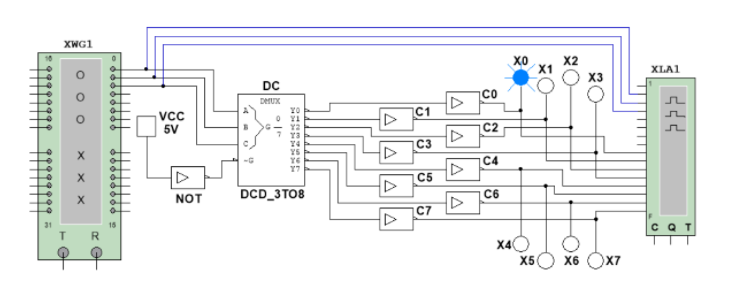
\includegraphics[width=0.8\textwidth]{pic2/1.png}
    \caption{}
\end{figure}

По результатам моделирования составим и заполним таблицу переключений 
функций $Y_i=(A_iB_iC_i;G_i)$ на выходах дешифратора $DC ~3\text{x}8$.

\begin{table}[h]
    \begin{center}
    \begin{tabular}{|l|l|l|l|l|l|l|l|l|}
    \hline
          & $X_0$ & $X_1$ & $X_2$ & $X_3$ & $X_4$ & $X_5$ & $X_6$ & $X_7$ \\ \hline
    $A_i$ &       & 1     &       & 1     &       & 1     &       & 1     \\ \hline
    $B_i$ &       &       & 1     & 1     &       &       & 1     & 1     \\ \hline
    $C_i$ &       &       &       &       & 1     & 1     & 1     & 1     \\ \hline
    \end{tabular}
\end{center}
\end{table}


\section{Задание 2}
Построим схему шифратора $CD$:


\begin{center}$y=(ab+\urcorner c)(\urcorner a+\urcorner b+c)(a+b+c)$\end{center}

\begin{figure}[H]
    \centering
    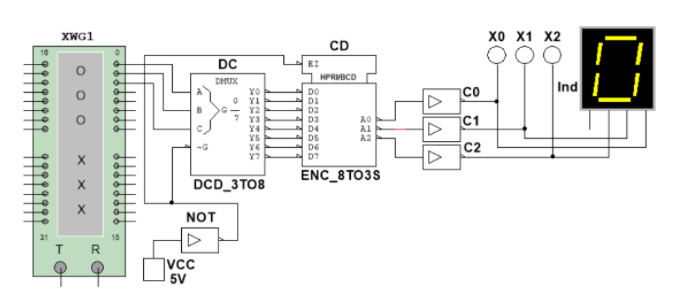
\includegraphics[width=0.8\textwidth]{pic2/2.png}
    \caption{}
\end{figure}

По результатам моделирования (по подсвечиванию пробников $X_0,X_1,X_2$ и 
показаниям индикатора $Ind$) составим и заполним таблицу переключений на выходе
шифратора $CD ~8\text{x}3$:

\begin{table}[h]
    \begin{center}
    \begin{tabular}{|l|l|l|l|}
    \hline
          & $A_i$ & $B_i$ & $C_i$ \\ \hline
    $X_0$ &       &       &       \\ \hline
    $X_1$ & 1     &       &       \\ \hline
    $X_2$ &       & 1     &       \\ \hline
    $X_3$ & 1     & 1     &       \\ \hline
    $X_4$ &       &       & 1     \\ \hline
    $X_5$ & 1     &       & 1     \\ \hline
    $X_6$ &       & 1     & 1     \\ \hline
    $X_7$ & 1     & 1     & 1     \\ \hline
    \end{tabular}
    \end{center}
\end{table}

Преобразуем схему дешифратора $DC~3 \text{x}8$ и шифратора $CD~8\text{x}3$ в схему
$DC ~2\text{x}4$ и шифратора $CD~4\text{x}2$, отсоединив провод $C$, подходящий
к дешифратору, и провод $A2$ с выхода шифратора, и составим таблицы переключений
дешифратора 2x4 и шифратора 4x2:

\begin{table}[H]
    \begin{center}
    \begin{tabular}{|l|l|l|l|l|}
    \hline
          & $X_0$ & $X_1$ & $X_2$ & $X_3$ \\ \hline
    $A_i$ &       & 1     &       & 1     \\ \hline
    $B_i$ &       &       & 1     & 1     \\ \hline
    \end{tabular}
    \end{center}
\end{table}

\begin{table}[H]
    \begin{center}
    \begin{tabular}{|l|l|l|}
    \hline
          & $A_i$ & $B_i$ \\ \hline
    $X_0$ &       &       \\ \hline
    $X_1$ & 1     &       \\ \hline
    $X_2$ &       & 1     \\ \hline
    $X_3$ & 1     & 1     \\ \hline
    \end{tabular}
    \end{center}
\end{table}

\section{Вывод}
В ходе лабораторной работы мы ознакомились с основными характеристиками логических
элементов, научились строить модели схем в специальном программном обеспечении,
а также, оперируя определенными ключами, перебрали возможные комбинации в
одной из реализации схем, что позволило получить ансамбль выходных данных
для всевозможных вариациях входных значений. Также ознакомились с основами
синтеза логических схем.

\section{Тестовые задания}

\subsection{Задание 1}
    Укажите признаки характеризующие основные логические элементы:
    
    \begin{enumerate}
        \item используя основные логические операции И, ИЛИ и НЕ, можно аналитически
        выразить любую сложную логическую функцию;
        \item минимальный логический базис составляют операции ИЛИ и НЕ или И и НЕ;
        \item входные и выходные сигналы логических элементов могут принимать
        только два значения: логическую 1 и логический 0;
    \end{enumerate}


\subsection{Задание 2}
    Укажите выражение логической функции двух переменных $x_1$ и $x_2$, реализуемой элементом «стрелка Пирса»:
    
    \begin{center}$y = \overline{x_1 + x_2}$\end{center}

\subsection{Задание 3}
     Укажите выражение логической функции двух переменных $x_1$ и $x_2$, реализуемой элементом «штрих Шеффера»:
    
    \begin{center}$y = \overline{x_1x_2}$\end{center}
    
\subsection{Задание 4}
     Укажите выражение логической функции трех переменных $a, b ~\text{и}~ c$, 
     записанной в совершенной дизъюнктивной нормальной форме (СДНФ):

    \begin{center}$y(a, b, c) = \overline{a}bc + a\overline{b}c + ab\overline{c} + abc$\end{center}

\subsection{Задание 5}
    Укажите элемент ИЛИ-НЕ:
    
    \begin{figure}[H]
        \centering    
        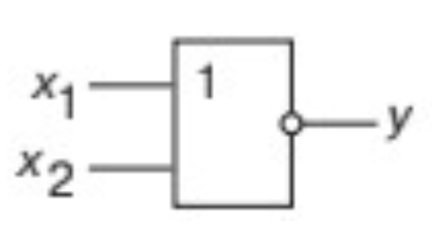
\includegraphics[width=0.4\textwidth]{pic1/3.png}
    \end{figure}

   
\subsection{Задание 6}
    Укажите элемент И:
    
    \begin{figure}[H]
        \centering
        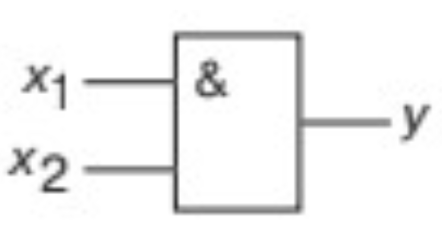
\includegraphics[width=0.4\textwidth]{pic1/4.png}
    \end{figure}

\subsection{Задание 7}
    Укажите значение функции $y = (ab + \overline{c})(\overline{a} + \overline{b})$ если $a = b = c = 1$:
    
    0

\end{document}